\chapter{Pattern size constrains}
In the previous chapter, we characterized what matrices avoiding small patterns look like. Their structure is very dependent of the pattern and the results are hard to generalize for arbitrary patterns. In this chapter, we will look for a more general property that restricts the complexity a class of matrices avoiding a given pattern can have.
\begin{defn}
In a matrix~$M\in\Mat$ a \emph{one-interval} in a row~$r$ is a sequence of one-entries in $M[\{r\},[c_1,c_2]]$ such that either $c_1=1$ or $M[r,c_1-1]$ is a zero-entry and at the same time either $c_2=n$ or $M[r,c_2+1]$ is a zero-entry. In other words, one-interval is an interval of one-entries bounded by the edge of matrix or zero-entries. We use the same name also for interval of one-entries in a column. In the same spirit we also define \emph{zero-interval} to be an interval of zero-entries bounded by one-entries or a edge of matrix.
\end{defn}
In Sections ref, it always holds that for a pattern~$P$ of size $k\times l$ any inclusion maximal matrix $M$ that avoids $P$ as an interval minor has at most $l-1$ one-intervals in each row and at most $k-1$ one-intervals in each column. A natural question is whether the size of a pattern indeed bounds the number of one-intervals of any inclusion maximal matrix that avoids it.

Before we start, let us present some useful notion. First of all, every time we speak about \emph{maximal} matrices from a class, we mean inclusion maximal -- it has no zero-entry that can be changed to a one-entry and still belong to the class. In terms of pattern avoidance maximal matrices are those for which a change of a zero-entry creates a mapping of the pattern (or possibly many mappings).
\begin{defn}
Let $P$ be a pattern, $e$ a one-entry of $P$, $M$ be a maximal matrix such that $\PnimM$ and $z$ arbitrary zero-interval of $M$. We say that $z$ \emph{is usable for} $e$ if there is a zero-entry contained in $z$ such that if we change it to a one-entry, it creates a mapping that uses the new one-entry to map $e$. Note that $z$ can be usable for many one-entries of $P$ at the same time. 
\end{defn}
\begin{defn}
Let $\mathcal{P}$ be a class of patterns. We say that $Av(\mathcal{P})$ is \emph{bounded} if there is a function dependent only on the size of patterns in $\mathcal{P}$ such that every maximal $M\in Av(\mathcal{P})$ has the number of one-intervals in each row and column bounded by the function. Otherwise, we say that $Av(\mathcal{P})$ is \emph{unbounded}. To denote the same situation, we also say that patterns in $\mathcal{P}$ are \emph{bounded} or \emph{unbounded}.
\end{defn}
\begin{defn}
Let $P\in\Pat$ be a pattern and $e$ any of its one-entries. We say that $e$ is \emph{row-bounded} if there is a function of $k$ and $l$ such that for each maximal matrix avoiding $P$ and each of its rows the number of zero-intervals that are usable for $e$ is bounded by the function. In symmetric way, we also define \emph{column-bounded} one-entries of $e$. We say that $e$ is \emph{bounded} if it is both row-bounded and column-bounded.
\end{defn}
Let us look on how definitions relate to each other. Let us have a pattern~$P$ and assume each of its one-entries is bounded. From the definition it immediately follows that $P$ is bounded and that is equivalent to saying that class $Av(P)$ is bounded. It also holds that if a one-entry of $P$ is row-bounded then the same one-entry of $P^T$ is column-bounded.

\section{Motivation}
\begin{thm}
Let $P\in\{0,1\}^{k\times2}$ and $M\in\Mat$ be a  maximal matrix such that $\PimM$, then $M$ contains at most one one-interval in each row.
\end{thm}
\begin{proof}
For contradiction, assume there are several one-intervals in the same row of $M$. Because $M$ is maximal avoiding $P$ as an interval minor, changing any one-entry~$e$ in between two consecutive one-intervals creates a mapping of the forbidden pattern. Such a mapping uses the changed one-entry to map some element $P[r',1]$ or $P[r',0]$. In the first case, the same mapping also works if we use any one-entry that is to the left from $e$ instead of $e$, which leads to $\PimM$ and therefore a contradiction. In the second case, the mapping can use any one-entry to the right from $e$ instead of $e$ and therefore, there is no mapping of $P$ to $M$ even if $e$ is a one-entry. That is a contradiction with $M$ being maximal.
\end{proof}
TO DO ref to what we proved by this
\begin{thm}
\label{smallintnum}
Let $P\in\{0,1\}^{k\times 2}$ and $M\in\Mat$ be a maximal matrix such that $\PimM$, then $M$ contains at most $2k+2$ one-intervals in each column.
\end{thm}
\begin{proof}
Given an arbitrary maximal matrix $M$ avoiding $P$ let us look at an arbitrary column $c$. For contradiction, assume it has at least $2k+3$ one-intervals which also means there are at least $2k+1$ zero-intervals in between. Since $P$ has at most $2k$ one-entries, from the Pigeonhole principle there are two zero-intervals usable for the same one-entry.

TO DO describe that mapping of the middle row is bounded by the edges of zero-interval and define the common mapping.
\end{proof}
\begin{cor}
Every $P\in\{0,1\}^{k\times 2}$ is bounded.
\end{cor}
We see that for patterns having only two rows or columns we can indeed bound the number of one-intervals of maximal matrices avoiding them. On the other hand, already for a pattern of size $3\times3$ we show that there are matrices with arbitrarily many intervals of one-entries and we cannot get their number smaller.

\section{Unbounded number of one-intervals}
\begin{thm}
\label{manyints}
Let $P=\smm{ &1& \\1& & \\ & &1}$. For every $n>1$ there is a maximal matrix $M$ avoiding $P$ as an interval minor having $n$ one-intervals ($P$ is unbounded).
\end{thm}
\begin{proof} Let $M$ be a $(2n-1)\times(2n-1)$ matrix described by the picture:
$$\smm{	1&0&1&0&1&\cdots&1&0&1&0&1\\
		 & & & & &\cdots& & &1&1&1\\
		 & & & & &\cdots& & &1&1&1\\
		 & & & & &\cdots&1&1&1& & \\
		 & & & & &\cdots&1&1&1& & \\
		\vdots&\vdots&\vdots&\vdots&\vdots&\iddots&\vdots&\vdots&\vdots&\vdots&\vdots\\
		 & &1&1&1&\cdots& & & & & \\
		 & &1&1&1&\cdots& & & & & \\
		1&1&1& & &\cdots& & & & & \\
		1&1&1& & &\cdots& & & & & \\
		 }$$
$\PnimM$ because we always need to map $P[2,1]$ and $P[3,3]$ to just one ``block'' of one-entries of $M$ which only leaves zero-entries where we need to map $P[1,2]$.

When we change any zero-entry of the first row into a one-entry (getting $M'$) we get a matrix containing a minor of $\{1\}^{3\times3}$; therefore, containing $P$ as an interval minor. In case $M$ is not maximal, we can add some more one-entries to make it maximal but it will still contain a row with $n$ intervals of one-entries.
\end{proof}
Not only $M$ is a maximal matrix avoiding $P$ but also avoiding any $P'\in\{0,1\}^{3\times3}$ such that $P\im P'$. Its rotations avoid rotations of $P$ and we can deduce that a big portion of patterns of size $3\times3$ are unbounded. Moreover, the result can be generalized also for bigger matrices. The pattern is so important that we call it $P_1$ for the rest of the chapter.
\begin{thm}
For every $P'$ such that $P_1\im P'$ and every $n>1$ there is a maximal matrix $M$ avoiding $P'$ as an interval minor having $n$ one-intervals.
\end{thm}
\begin{proof}
First, assume there is a mapping of $P_1$ into $P'\in\Pat$ that assigns a one-entry of the first row to $P_1[1,2]$, a one-entry of the first column to $P_1[2,1]$ and a one-entry of the last row and column to $P_1[3,3]$. Then, we can construct a similar matrix as we did in the proof of Theorem~\ref{manyints} avoiding $P'$ but after changing any zero-entry of the first row it contains the whole $\{1\}^{k\times l}$.

Let $P'$ be any pattern containing $P$ without additional restrictions. Let $P'[r_1,c_1],P'[r_2,c_2]$ and $P'[r_3,c_3]$ be one-entries of $P'$ that can be used to map $P_1[1,2],P_1[2,1]$ and $P_1[3,3]$ to it respectively. Then we take a submatrix $P'':=P'[[r_1,r_3],[c_2,c_3]]$. Such a matrix fulfills assumptions of the more restricted case stated at the beginning of the proof and we can find a maximal matrix $M'$ avoiding $P''$ having $n$ one-intervals. We construct $M$ from $M'$ by simply adding new rows and columns, all containing one-entries. We add $r_1-1$ rows in front of the first row and $k-r_3$ rows behind the last row. We also add $c_2-1$ columns in front of the first column and $l-c_3$ columns behind the last column. Constructed matrix $M$ avoids pattern $P'$ as its submatrix $P''$ cannot be mapped to $M$ without added rows and columns. At the same time, any change of a zero-entry of the $r_1$-th row of $M$ to one-entry creates a copy of ${1}^{k\times l}$ so the changed matrix contains $P'$.
\end{proof}

\section{Bounded number of one-intervals}
What makes it even more interesting is that any pattern avoiding all rotations of $P_1$ is already bounded. To prove that we need a few partial results.
\begin{thm}
Let $P$ be a pattern avoiding all rotations of $P_1$, then $P$:
\begin{enumerate}
	\item contains one non-empty line or
	\item contains two non-empty lines or
	\item contains three non-empty lines or
	\item avoids $\smm{1& \\ &1}$ or $\smm{ &1\\1& }$.
\end{enumerate}
\end{thm}
\begin{proof}
Assume $P$ has four one-entries that do not share any row or column. Then those one-entries induce a $4\times4$ permutation inside $P$ and because $P$ does not contain any rotation of $P_1$, the induced permutation is either $1234$ or $4321$. Without loss of generality, assume is the the first case and denote the one-entries by $e_1,e_2,e_3$ and $e_4$.

For contradiction with the statement, assume $P$ also contains $P'=\smm{1& \\ &1}$. Clearly, any one-entry from $e_1,e_2,e_3$ and $e_4$ cannot be a part of any mapping of $P'$ because it would introduce a mapping of a rotation of $P_1$. Let $e_2=P[r_2,c_2]$ and $e_3=P[r_3,c_3]$. First, the submatrix $P[[r_2],[c_2,l]]$ does not contain $P'$ because then this copy of $P'$ together with $e_4$ would give us a rotated copy of $P_1$. Symmetrically, $P[[r_3,k],[c_3]]$ does not contain $P'$. Also, $P[[r_3-1],[c_3-1]]$ and $P[[r_2+1,k],[c_2+1,l]]$ are empty (else they would together with $e_2$ and $e_3$ give us a mapping of a rotation of $P_1$). Up to rotation, the only possible way to have $P'\im P$ is that the top one-entry of $P'$ is in the submatrix $P[[r_3-1],[c_2,c_3-1]]$ but then this entry together with $e_1$ and $e_3$ give us a mapping of a rotation of $P_1$ which is a contradiction.
\end{proof}

Now comes the hard part. For each group of patterns, we need to prove all of them are bounded.

%%%%%%%%%%%%%%%%%%%%%%%%%%%%%%%%%%%%%%%%%%%%%%%%%% one non-empty line
\begin{lemma}
Let $P\in\Pat$ be a pattern having only one non-empty line. Then for every maximal matrix $M\in\Mat$ avoiding $P$ the number of one-intervals in each row and column is bounded by $O(k+1)$. 
\end{lemma}
\begin{proof}
Let the non-empty line of $P$ be a row~$r$. Since $M$ is maximal, submatrices $M[[r-1],[n]]$ and $M[[m-r+1,m],[n]]$ contain no zero-entry and each of their rows contains just one interval of one-entries. If we look at any other row, it cannot contain $k$ one-entries, so the maximum number of one-intervals is $k-1$.

Let us look on an arbitrary column~$c$ of $M$. If there is at least one one-entry in $M[[r,m-r],c]$ then because $M$ is maximal, the whole column is made of one-entries. Otherwise, there are two intervals of one-entries -- $M[[r-1],c]$ and $M[[m-r,m],c]$.
\end{proof}

%%%%%%%%%%%%%%%%%%%%%%%%%%%%%%%%%%%%%%%%%%%%%%%%%% two non-empty lines
\begin{lemma}
Let $P\in\Pat$ be a pattern having two non-empty lines. Then for every maximal matrix $M\in\Mat$ avoiding $P$ the number of one-intervals in each row and column is bounded by $2k+2l+3$. 
\end{lemma}
\begin{proof}
First we assume the two non-empty lines of $P$ are rows $r_1<r_2$ (or symmetrically columns). From Observation~\ref{emptyrows} and maximality of $M$ we have that $M[[r_1-1],[n]]$ and $M[[m-r_2+1,m],[n]]$ contain no zero-entry. Therefore, we may restrict ourselves to case $r_1=1$ and $r_2=k$. From Theorem~\ref{smallintnum} we know that every maximal $N$ avoiding $P[\{r_1,r_2\},[n]]$ has at most $2k+3$ one-intervals of one-entries in each row and at most $1$ one-interval in each column. From Theorem~\ref{emptymiddle} we also know that for given $M$ there is a  maximal $N$ avoiding $P[\{r_1,r_2\},[n]]$ such that $M$ is submatrix of shifted and OR-ed copies of $N$. Since $M$ is maximal it is equal to those shifted and OR-ed copies of $N$ and since the number of one-intervals of $N$ is bounded, so is the number of one-intervals of $M$.

\begin{figure}[!ht]
\centering
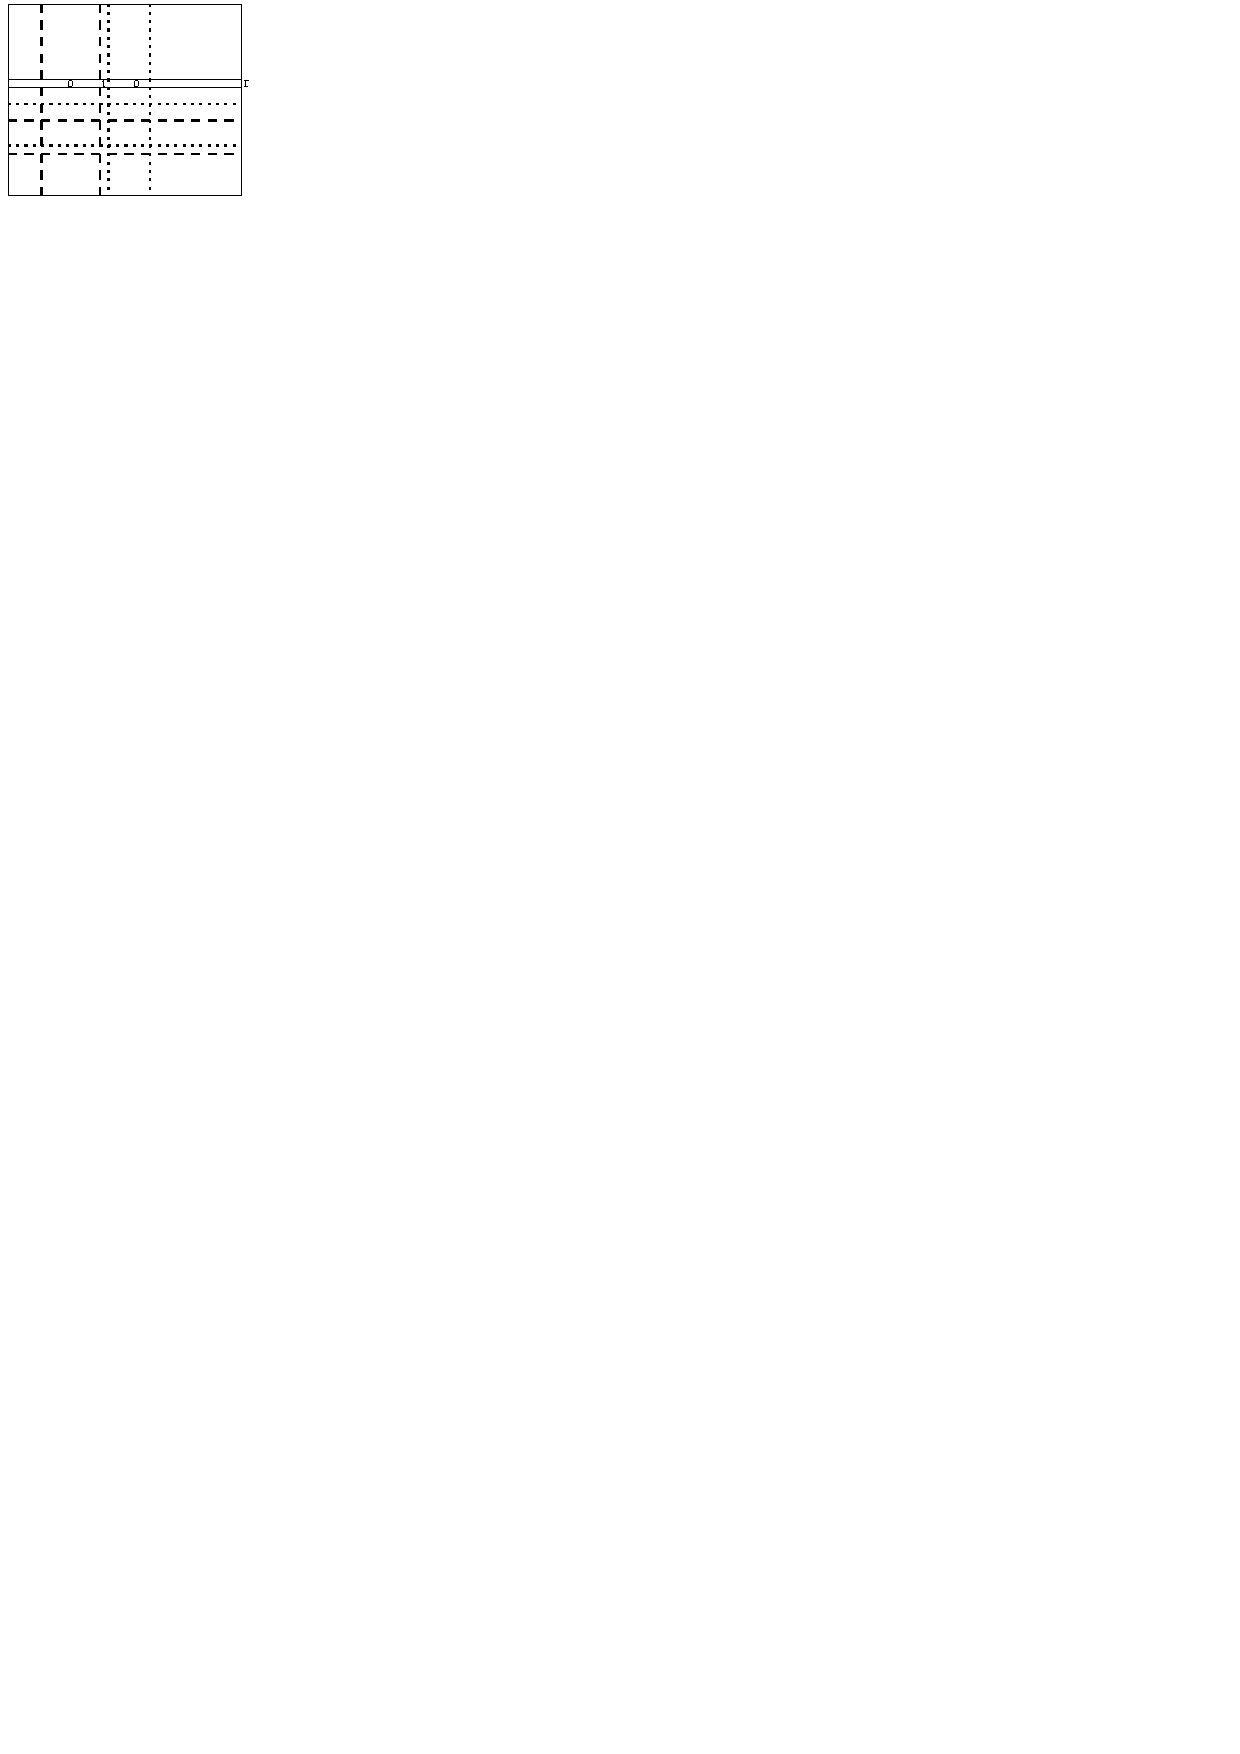
\includegraphics[height=60mm]{img/twolines.pdf}
\caption{Dashed and dotted lines resembling two different mappings of a forbidden pattern, where two horizontal lines show the boundaries of the mapping of row~$r$ and the vertical lines show boundaries of the mapping of column~$c$.}
\label{twolines}
\end{figure}
Assume the two non-empty lines of $P$ are row~$r$ and column~$c$. Because the proof is symmetric, we only show the bound for rows. Let us take an arbitrary row of $M$ an look at its zero-intervals. For every one-entry~$e$ of the pattern except those in the $r$-th row, there is at most one zero-interval usable for $e$. For contradiction, assume there are two such zero-intervals. Let Figure~\ref{twolines} illustrate the situation where dashed  and dotted lines form a partitioning of the minor $P$ in $M$ when a respective zero-entry of our two zero-intervals is changed to a one-entry. When we take the outer two vertical and horizontal lines, we get a mapping of $P$ that can use an existing one-entry in between the two zero-intervals to also map $e$. This gives us a contradiction with $\PnimM$. Therefore, for every one-entry~$e$ of $P$ from the $r$-th row there is at most one zero-interval usable for it. This gives us the bound.
\end{proof}

To argue about the last two cases more easily, we introduce two helpful lemmata.

%%%%%%%%%%%%%%%%%%%%%%%%%%%%%%%%%%%%%%%%%%%%%% Lemma H
\begin{lemma}
\label{lemmaH}
Let $P\in\Pat$ be a pattern looking like one of the matrices in Figure~\ref{lemmaHfig}. Then every one-entry from row~$r_2$ in columns $c_1$ to $c_2$ is row-bounded.

\begin{figure}[!ht]
\centering
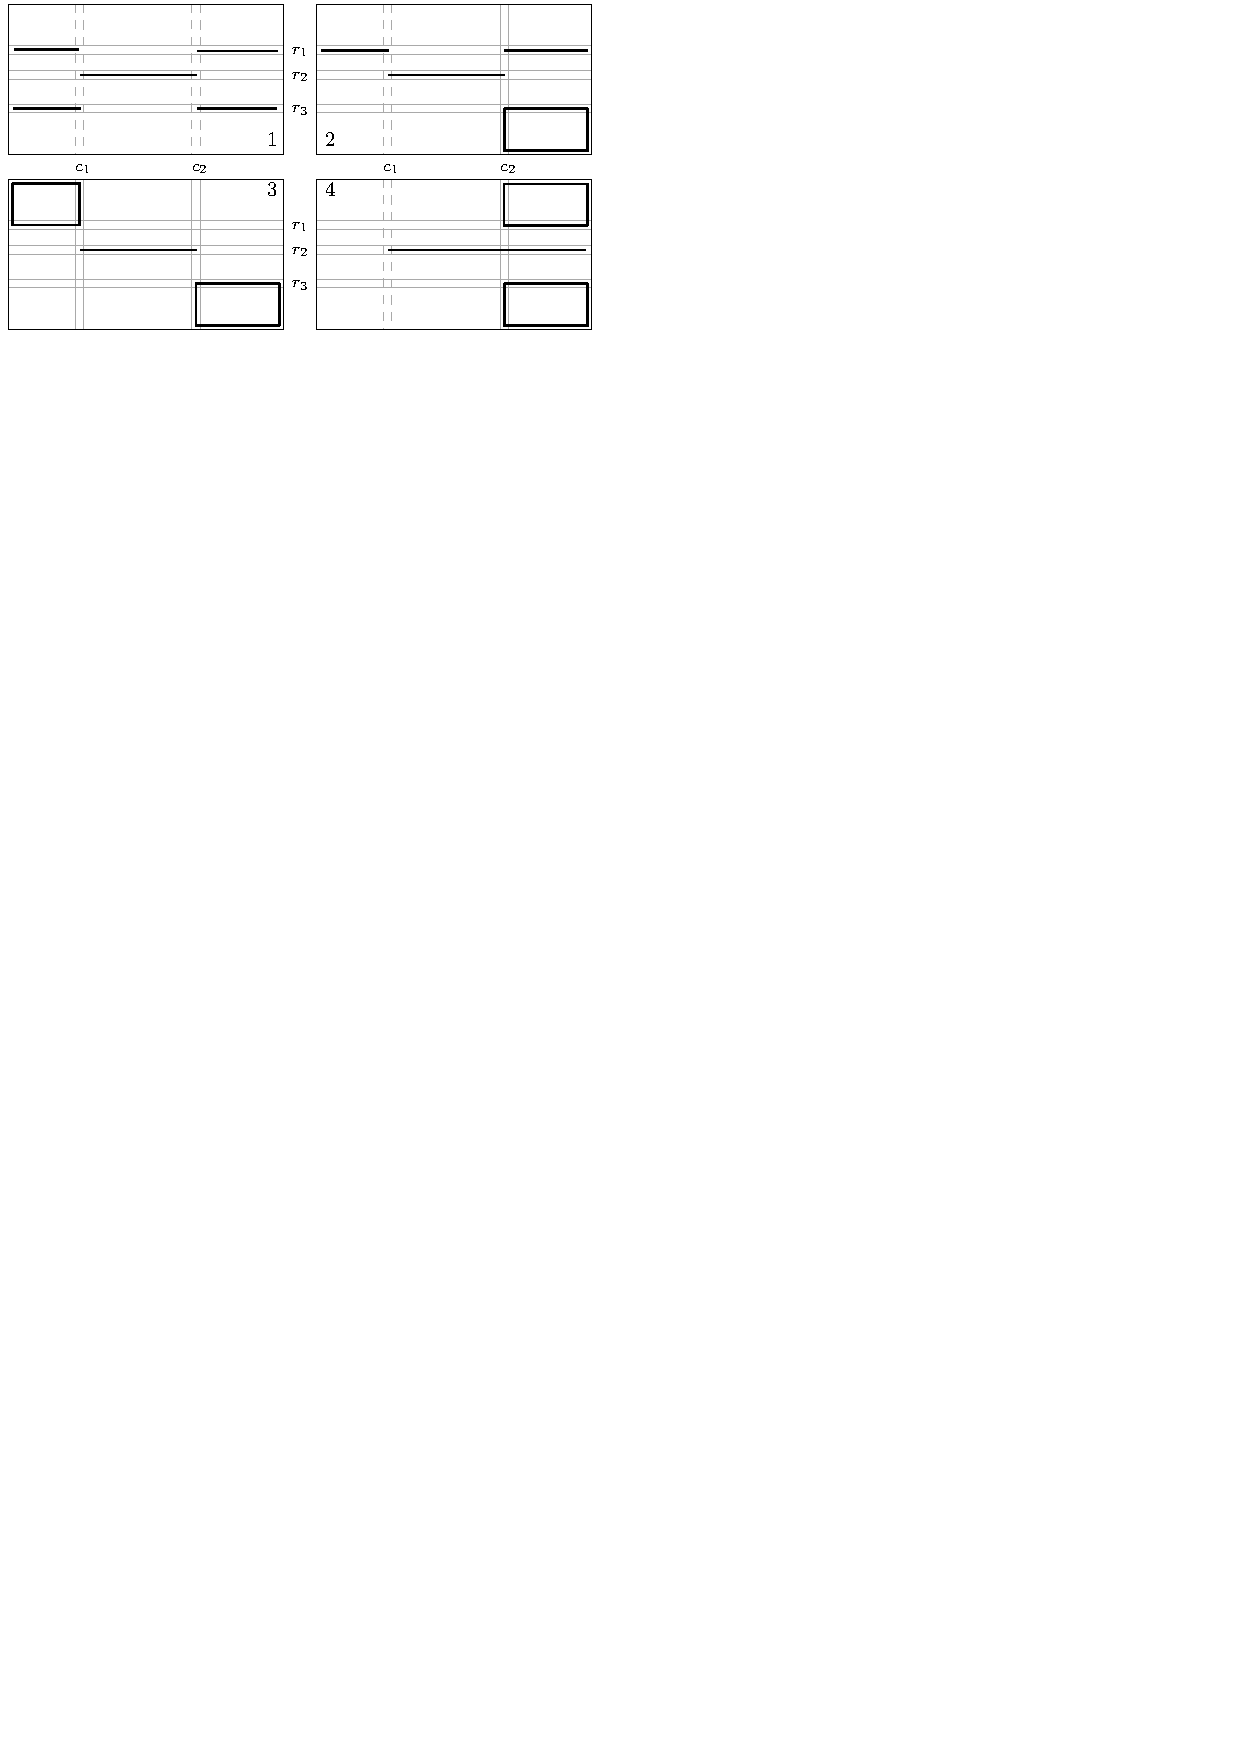
\includegraphics[width=\textwidth]{img/lemmaH.pdf}
\caption{Patterns for which one-entries in row~$r_2$ are row-bounded. One-entries may only be in the areas enclosed by bold lines.}
\label{lemmaHfig}
\end{figure}
\end{lemma}
\begin{proof}
Let $P$ be any of the first three described patterns and let $k'=c_2-c_1$. We even show that for each one-entry $e$ from row~$r_2$ and every $M$ maximal matrix avoiding $P$ there is at most $k'$ zero-intervals for which it is usable. For contradiction assume there is a row~$r$ with $k'+1$ zero-intervals usable for $e$. It follows that there are at least $k'$ one-entries in between two most distant zero-intervals $z_1$ and $z_2$. Therefore, the whole row~$r_2$ can be mapped just to $r$. Since changing a zero-entry of $z_1$ to a one-entry to which $e$ can be mapped, there is a partitioning of $M$ where all one-entries from columns $1$ to $c_1$ are mapped to columns before $z_1$ and similarly all one-entries from columns $c_2$ to $l$ are mapped to columns past $z_2$. To partition rows, we can simply map rows from $r_1+1$ to $r_3-1$ around row $r$ one to one and use the rest to find enough one-entries for the one-entries of $P$. The partitioning using those one-entries and one-entries from $r$ to map one-entries of $r_2$ together give us $\PimM$ and a contradiction.

Make a picture? The explanation is not clear at all.

Let us look on the fourth case. For $i$-th one-entry in row~$r_2$ (ordered from left to right and only considering those in columns $c_1$ to $c_2$) no zero-interval of a maximal matrix avoiding the pattern cannot have $i$ one-entries to the left of it and so each such one-entry is bounded by $i\geq l$.
\end{proof}

%%%%%%%%%%%%%%%%%%%%%%%%%%%%%%%%%%%%%%%%%%%%%% First non-empty column bounded
\begin{lemma}
\label{lemmaFirst}
Let $P$ be a pattern and $c$ be its first non-empty column. Then every one-entry from $c$ is row-bounded.
\end{lemma}

\begin{proof}
The results follows immediately from the fourth case of Lemma~\ref{lemmaH} when there are no one-entries in columns before $c_2$.
\end{proof}

%%%%%%%%%%%%%%%%%%%%%%%%%%%%%%%%%%%%%%%%%%%% Lemma I
\begin{lemma}
\label{lemmaI}
Let $P\in\Pat$ be a pattern looking like one of the matrices in Figure~\ref{lemmaIfig}. Then every one-entry from column~$c$ in rows $r_1$ to $r_2$ is row-bounded.
\begin{figure}[!ht]
\centering
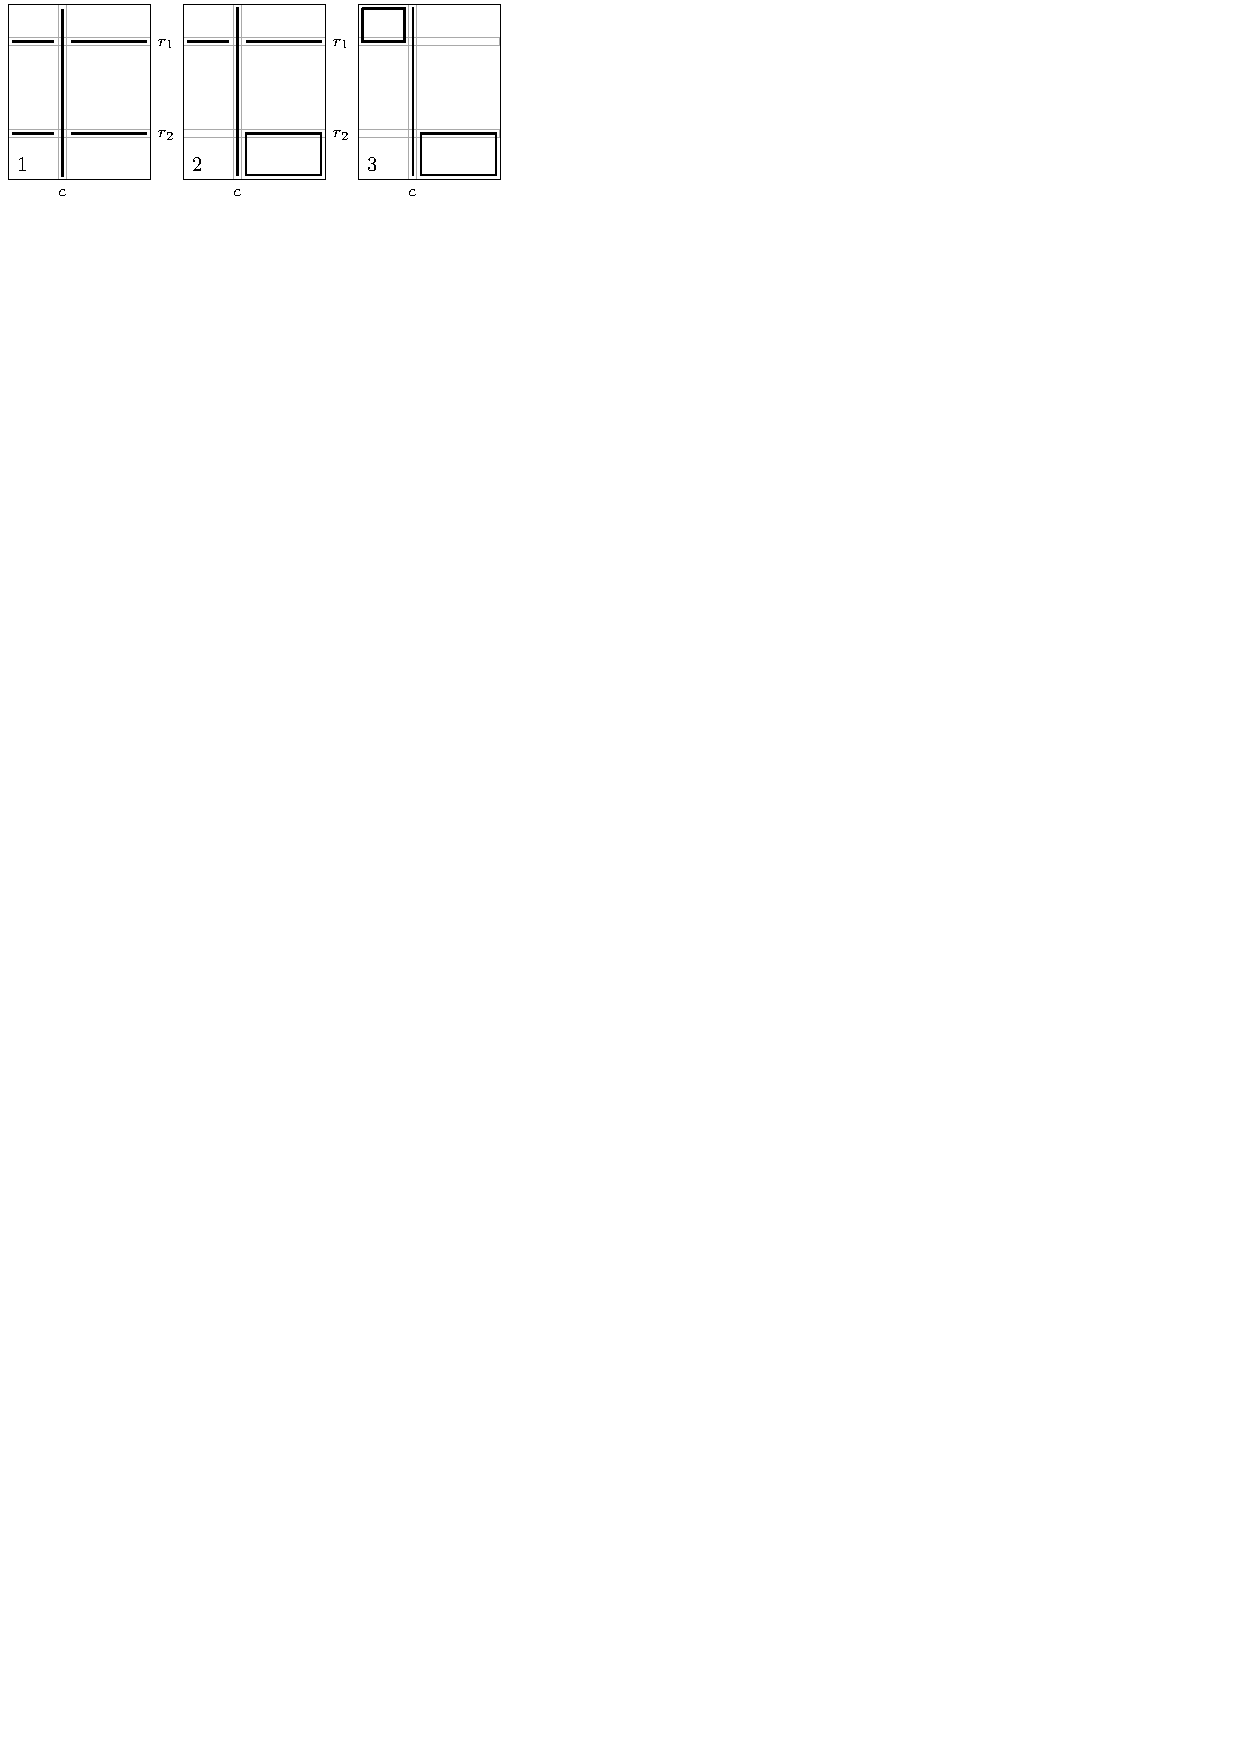
\includegraphics[width=120mm]{img/lemmaI.pdf}
\caption{Patterns for which one-entries in column~$c$ are row-bounded. One-entries may only be in the areas enclosed by bold lines.}
\label{lemmaIfig}
\end{figure}
\end{lemma}
\begin{proof}
Let $P$ be any of the described patterns. We even show that for each one-entry $e$ from row~$r_2$ and every $M$ maximal matrix avoiding $P$ there is at most one zero-interval for which it is usable. For contradiction assume there is a row~$r$ with two zero-intervals usable for $e$.

Again a picture needed -- take the closer partitioning and it is done
\end{proof}

%%%%%%%%%%%%%%%%%%%%%%%%%%%%%%%%%%%%%%%%%% walking patterns
\begin{lemma}
\label{lemmaWalkPat}
Let $P\in\Pat$ be a pattern avoiding $\smm{0&1\\1&0}$ (or $\smm{1&0\\0&1}$). Then for every maximal matrix $M\in\Mat$ avoiding $P$ the number of one-intervals in each row and column is bounded.
\end{lemma}
\begin{proof}
From Theorem~\ref{walkingthm} we know that $P$ is a walking pattern. Every one-entry of $P$ satisfies either conditions of the third case of Lemma~\ref{lemmaH} or it satisfies conditions of the third case of Lemma~\ref{lemmaI} and therefore is row-bounded. To prove it is also column-bounded, we can look at $P^T$ and show that its one-entries are row-bounded. Since it is again a walking pattern, we can use the same arguments.
\end{proof}

%%%%%%%%%%%%%%%%%%%%%%%%%%%%%%%%%%%%%%%%%%% three non-empty lines - it is super long
\begin{lemma}
Let $P\in\Pat$ be a pattern having three non-empty lines and avoiding all rotations of $P_1$. Then for every maximal matrix $M\in\Mat$ avoiding $P$ the number of one-intervals in each row and column is bounded. 
\end{lemma}
\begin{proof}
First of all, if $P$ avoids $\smm{0&1\\1&0}$ or $\smm{1&0\\0&1}$ we can use Lemma~\ref{lemmaWalkPat}. Without loss of generality we assume it contains both but avoids every rotation of $P_1$.

Let us prove that each pattern having one-entries in three rows is bounded. If all one-entries are in up to two columns then we are again done. Therefore, $P$ has one-entries in at least three columns and so it contains a three by three permutation matrix as a submatrix (or an interval minor). Since rotations of $P_1$ are avoided, that permutation is either 123 or 321 and without loss of generality we assume the first case. In Figure~\ref{threelinesfig} we see the structure of each such pattern. Capital letters stand for one-entries of the permutation, letters $a-f$ stand each for a potential one-entry and greek letters stand each for a potential sequence of one-entries and zero-entries. Everything else is zero. Not all one-entries can be present at the same time, because that would create a mapping of $P_1$ or its rotation and we also need to find $\smm{1&0\\0&1}$. The following analysis will only use hereditary arguments. This mean that if we prove $P$ is bounded, we also prove that each submatrix of $P$ is bounded. With this in mind, we restrict ourselves to maximal patterns.
\begin{itemize}
	\item $\gamma$ contains a one-entry $\Rightarrow f=0\Rightarrow$ because $\smm{1&0\\0&1}$ needs to be there it holds $a=1\Rightarrow\alpha=0$
		\begin{itemize}
			\item $d=1\Rightarrow b=0,\ \beta=0,\ e=0,\ c=?$:\\
				Lemma~\ref{lemmaH} (case 4): one-entries in $c,C,\gamma$ are row-bounded.\\
				Lemma~\ref{lemmaFirst}: $a$ and $A$ are row-bounded.\\
				Lemma~\ref{lemmaI} (case 1): $d$ and $B$ are row-bounded.\\
				
				Lemma~\ref{lemmaFirst}: all one-entries except for $B$ are column-bounded.\\
				Lemma~\ref{lemmaH} (case 1): $B$ is column-bounded.
			\item $d=0$
				\begin{itemize}
					\item $c=1\Rightarrow\beta=0,\ e=0,\ b=?$:\\
						Lemma~\ref{lemmaH} (case 4): one-entries in $c,C,\gamma$ are row-bounded.\\
						Lemma~\ref{lemmaFirst}: $a,b,A$ are row-bounded.\\
						Lemma~\ref{lemmaH} (case 1): $B$ is row-bounded.\\
						
						Lemma~\ref{lemmaFirst}: one-entries in the first and the third non-empty rows are column-bounded.\\
						Lemma~\ref{lemmaH} (case 2): $b,B$ are column-bounded.
					\item $c=0\Rightarrow$ in the maximal case $b=1,\ e=1,\ \gamma$ contains a one-entry:\\
						Lemma~\ref{lemmaH} (case 4): one-entries in $c,C,\gamma$ are row-bounded.\\
						Lemma~\ref{lemmaFirst}: one-entries in the first non-empty column are row-bounded.\\
						Lemma~\ref{lemmaH} (case 1): one-entries in the middle non-empty row are row-bounded.\\
						
						Lemma~\ref{lemmaFirst}: one-entries in the first and the third non-empty rows are column-bounded.\\
						Lemma~\ref{lemmaI} (case 2): one-entries in the middle non-empty row are column-bounded.
				\end{itemize}
		\end{itemize}
	\item $\gamma=0$
		\begin{itemize}
			\item $\alpha$ contains a one-entry $\Rightarrow a=0,\ b=0$:\\
				Every such pattern has already been dealt with as we can rotate it by 180 degrees, map $A$ and $\alpha$ to $\gamma$, map $d$ to $C$ and so on.
			\item $\alpha=0$:\\
				Without loss of generality, we can assume that $a=1$, because there needs to be $\smm{0&1\\1&0}$ and if we set $a=0$, it must hold $f=1$ and then we can just rotate the pattern by 180 degrees and get the case $a=1$.
				\begin{itemize}
					\item $d=1\Rightarrow b=0,\ e=0,\ \beta=0,\ c=?,\ f=?$:\\
						Lemma~\ref{lemmaFirst}: $a,f,A$ and $C$ are row-bounded.\\
						Lemma~\ref{lemmaI} (case 1): $c,d$ and $B$ are row-bounded.\\
						
						Lemma~\ref{lemmaFirst}: one-entries in the first and third non-empty rows are column-bounded.\\
						Lemma~\ref{lemmaH} (case 1): $B$ is column-bounded.
					\item $d=0$
						\begin{itemize}
							\item $e=1\Rightarrow c=0,\ b=?,\ f=?$:\\
								Since $\alpha=0$ it follows that if there is a one-entry in $\beta$ only if it can be in $e$.
								
								Lemma~\ref{lemmaFirst}: $a,f,A$ and $C$ are row-bounded.\\
								Lemma~\ref{lemmaH} (case 1): one-entries in $b,e,B$ and $\beta$ are row-bounded. \\
								
								Lemma~\ref{lemmaFirst}: $a,f,A$ and $C$ are column-bounded.\\
								Lemma~\ref{lemmaI} (case 1): one-entries in $b,e,B$ and $\beta$ are column-bounded.
							\item $e=0$:\\
								We can assume $c=1$ as else $e$ can be 1 and we have already dealt with that case. We can also assume $b=1$ since otherwise, we would have a submatrix of the case dealt with when $d=1$:\\
								Lemma~\ref{lemmaFirst}: $a,b$ and $A$ are row-bounded.\\
								Lemma~\ref{lemmaH} (case 4): $c$ and $C$ are row-bounded.\\
								Lemma~\ref{lemmaH} (case 1): $B$ is row-bounded.\\
										
								Because the pattern is symmetric, it is also column-bounded.
						\end{itemize}
				\end{itemize}
		\end{itemize}
\end{itemize}
The same analysis also proves that if the pattern with the same restrictions only has three non-empty column it is bounded.
\begin{figure}[!ht]
	\centering
	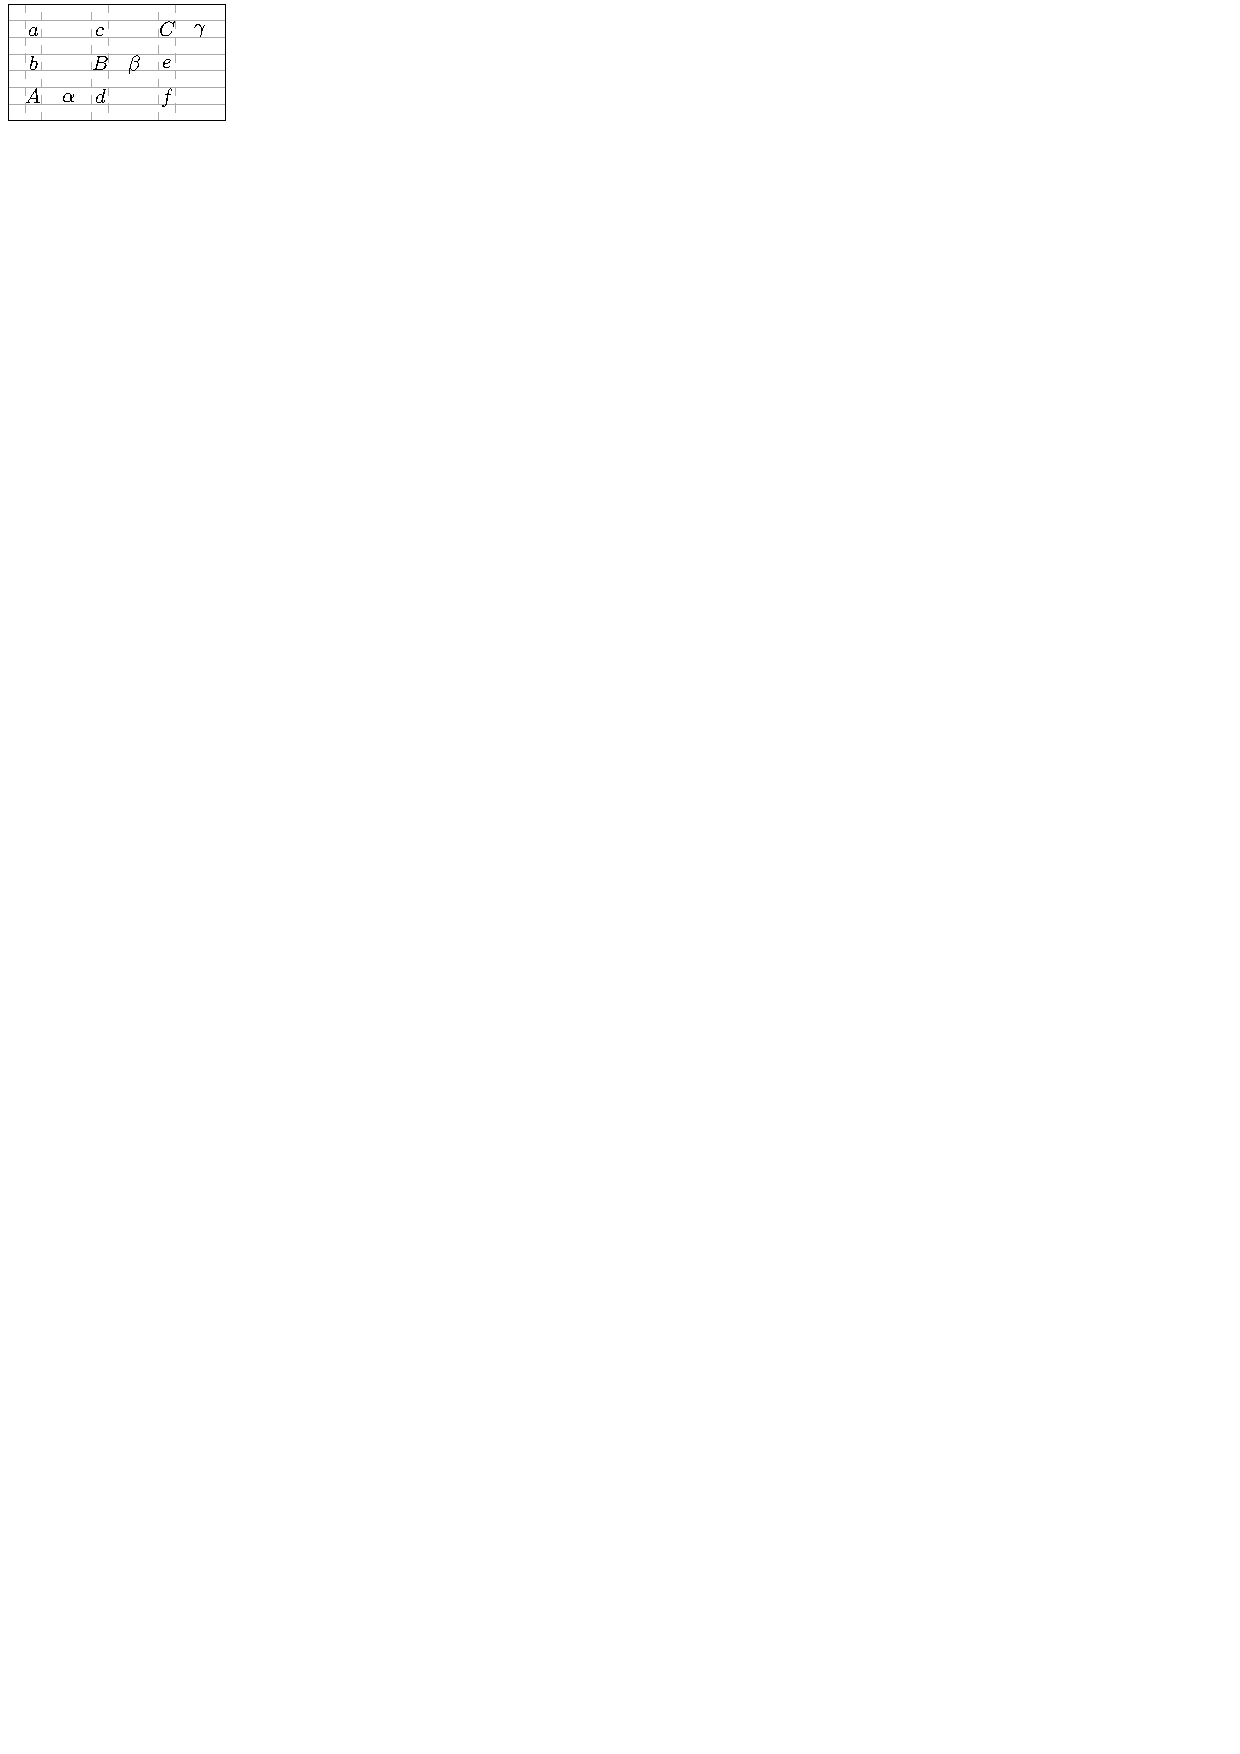
\includegraphics[width=70mm]{img/threelines.pdf}
	\caption{Structure of a pattern only having three non-empty rows and avoiding all rotations of $P_1$.}
	\label{threelinesfig}
\end{figure}

Let us now look at the case where the pattern that only have one-entries in either one of two rows $r_1,r_2$ or one column $c_1$. Without loss of generality we again assume permutation 123 is present and we distinguish three cases. Consider Figure~\ref{twoplusonefig}:
\begin{itemize}
\item $C$ lies in column~$c_1$
	\begin{itemize}
		\item $a=1\Rightarrow b=0,\ \alpha=0$ and everything else can be one:\\
			Lemma~\ref{lemmaH} (case 2): one-entries in $a,c,B$ and $\beta$ are row-bounded.\\
			Lemma~\ref{lemmaFirst}: all other one-entries are row-bounded.\\
			
			Lemma~\ref{lemmaH} (case 4): one-entries in $c,C$ and $\gamma$ are column-bounded.\\
			Lemma~\ref{lemmaI} (case 1): one-entries in $a,c,B$ and $\beta$ are column-bounded.\\
			Lemma~\ref{lemmaFirst}: $d$ and $A$ are column-bounded.
		\item $a=0$ and everything else can be one:\\
			Lemma~\ref{lemmaH} (case 4): one-entries in $b,A$ and $\alpha$ are row-bounded.\\
			Lemma~\ref{lemmaH} (case 2): one-entries in $c,B$ and $\beta$ are row-bounded.\\
			Lemma~\ref{lemmaFirst}: one-entries in $c,d,C$ and $\gamma$ are row-bounded.\\
			
			Lemma~\ref{lemmaH} (case 4): one-entries in $c,C$ and $\gamma$ are column-bounded.\\
			Lemma~\ref{lemmaI} (case 2): one-entries in $c,B$ and $\beta$ are column-bounded.\\
			Lemma~\ref{lemmaFirst}: one-entries in $b,d,A$ and $\alpha$ are column-bounded.			
	\end{itemize}
\item $B$ lies in column~$c_1$
	\begin{itemize}
		\item $a=1\Rightarrow\alpha=0$
			\begin{itemize}
				\item $d=1\Rightarrow\gamma=0$:\\
					Lemma~\ref{lemmaI} (case 1): all one-entries in column $c_1$ are row-bounded.\\
					Lemma~\ref{lemmaFirst}: all other one-entries are row-bounded.\\
					
					Lemma~\ref{lemmaH} (case 1): all one-entries in column $c_1$ are column-bounded.\\
					Lemma~\ref{lemmaFirst}: all other one-entries are column-bounded.
				\item $d=0$:\\
					Lemma~\ref{lemmaI} (case 1): all one-entries in column $c_1$ are row-bounded.\\
					Lemma~\ref{lemmaFirst}: $a$ and $A$ are row-bounded.\\
					Lemma~\ref{lemmaH} (case 4): one-entries in $C$ and $\gamma$ are row-bounded.\\
					
					Lemma~\ref{lemmaH} (case 1): all one-entries in column $c_1$ are column-bounded.\\
					Lemma~\ref{lemmaFirst}: all other one-entries are column-bounded.
			\end{itemize}
		\item $a=0$
			\begin{itemize}
				\item $d=1\Rightarrow\gamma=0$:\\
					Lemma~\ref{lemmaI} (case 1): all one-entries in column $c_1$ are row-bounded.\\
					Lemma~\ref{lemmaFirst}: $d$ and $C$ are row-bounded.\\
					Lemma~\ref{lemmaH} (case 4): one-entries in $A$ and $\alpha$ are row-bounded.\\
					
					Lemma~\ref{lemmaH} (case 1): all one-entries in column $c_1$ are column-bounded.\\
					Lemma~\ref{lemmaFirst}: all other one-entries are column-bounded.
				\item $d=0$:\\
					Lemma~\ref{lemmaI} (case 1): all one-entries in column $c_1$ are row-bounded.\\
					Lemma~\ref{lemmaH} (case 4): one-entries in $A,C,\alpha$ and $\gamma$ are row-bounded.\\
					
					Lemma~\ref{lemmaH} (case 1): all one-entries in column $c_1$ are column-bounded.\\
					Lemma~\ref{lemmaFirst}: all other one-entries are column-bounded.
			\end{itemize}
	\end{itemize}
\item $A$ lies in column~$c_1$:\\
	This is the first situation rotated by 180 degrees.
\end{itemize}
The same analysis also proves that if one-entries of a pattern with the same restrictions are in one row or two columns then the pattern it is bounded.
\begin{figure}[!ht]
	\centering
	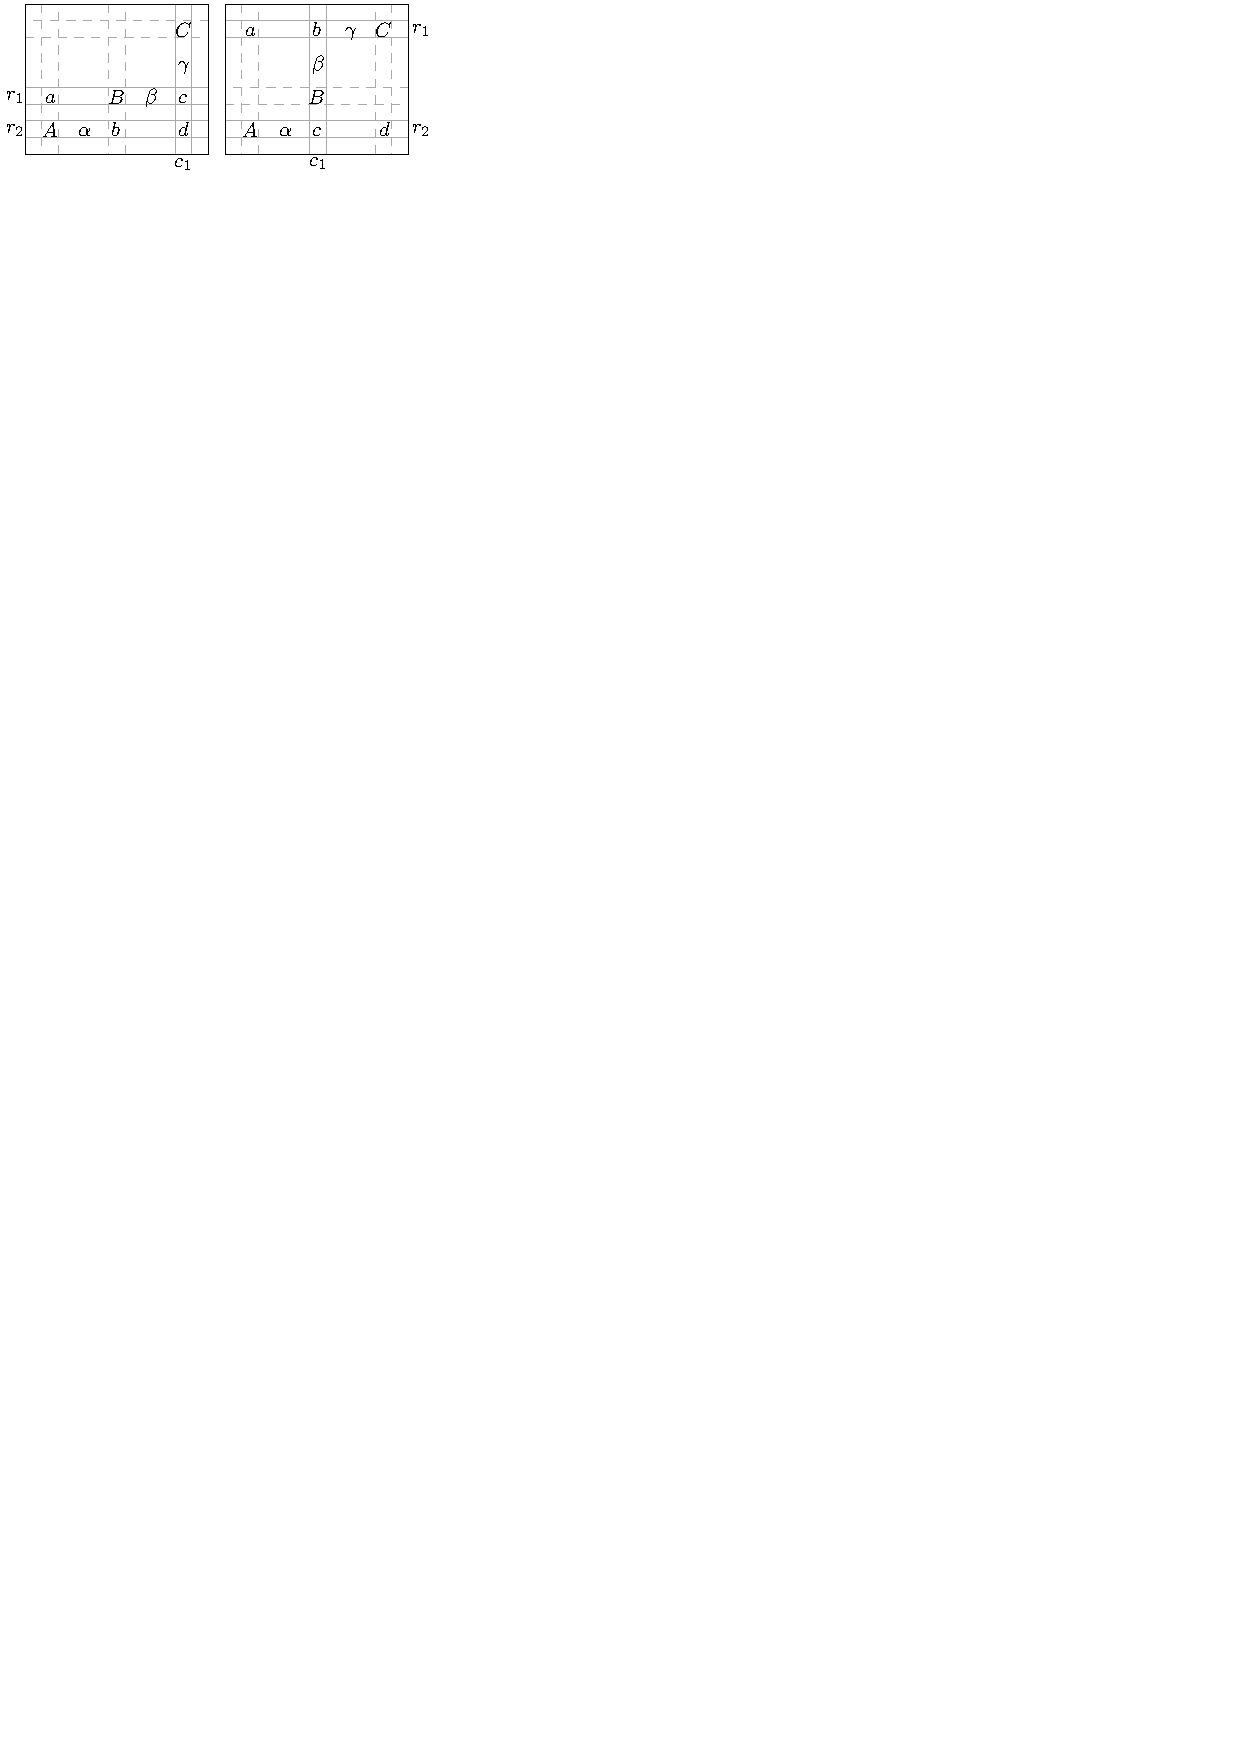
\includegraphics[width=120mm]{img/twoplusone.pdf}
	\caption{Structure of a pattern only having one-entries in two rows and one column that avoids all rotations of $P_1$.}
	\label{twoplusonefig}
\end{figure}
\end{proof}

Combining all the lemmata we finally get the following result.

\begin{thm}
Let $P$ be a pattern avoiding all rotations of $P_1=\smm{ &1& \\1& & \\ & &1}$, then $P$ is bounded.
\end{thm}

\section{Chain rules}
\begin{thm}
Let $\mathcal{P}$ and $\mathcal{Q}$ be finite classes of patterns. If both $\mathcal{P}$ and $\mathcal{Q}$ are bounded then $Av(\mathcal{P}\cup\mathcal{Q})$ is bounded.
\end{thm}
\begin{proof}
For a bounded pattern $P$, let $f(P)$ be a bound of the number of one-intervals of any maximal matrix avoiding $P$. For $\mathcal{P}$ let $f(\mathcal{P})=\sum_{P\in\mathcal{P}}f(P)$. Let $M$ be a maximal matrix avoiding $\mathcal{P}\cup\mathcal{Q}$ and take the line with the highest number of one-intervals. For every $P\in\mathcal{P}\cup\mathcal{Q}$ there is at most $f(P)+1$ zero-intervals usable for $P$'s one-entries. For contradiction assume there are more and change all zero-entries that are not usable for $P$'s one-entries with one-entries. This way we end up with a maximal matrix avoiding $P$ and a contradiction to $f(P)$ being the bound on the number of one-intervals of such matrix.

Together we then have $f(\mathcal{P}\cup\mathcal{Q})\geq f(\mathcal{P})+|P|+f(\mathcal{Q})+|Q|+1$ and since all numbers are finite, we have that $\mathcal{P}\cup\mathcal{Q}$ is bounded.
\end{proof}
Using induction, we can show that also a union of finite number of bounded classes of finite size are bounded. Interestingly enough, unbounded classes are not closed the same way.

\begin{fct}[Higman's lemma]
Let $A$ be a finite alphabet and $A^*$ be a set of finite sequences over $A$. Then $A^*$ is well quasi ordered with respect to the subsequence relation.
\end{fct}
\begin{thm}
$Av\left(\smm{ &1& \\1& & \\ & &1},\smm{ &1& \\ & &1\\1& & },\smm{1& & \\ & &1\\ &1& },\smm{ & &1\\1& & \\ &1& }\right)$ is bounded. Moreover, every subclass is bounded.
\end{thm}

\begin{obs}
There exists a non-trivial bounded pattern~$P$ having an unbounded subset of $Av(P)$.
\end{obs}
\begin{proof}
Let $P=I_n$ (identity matrix) for $n>3$. From Lemma~\ref{lemmaWalkPat} we have that $P$ is bounded. On the other hand, $Av(I_n,P_1)$ is unbounded, because the construction used in the proof of Theorem~\ref{manyints} also works for this class.
\end{proof}

Open questions:
\begin{itemize}
	\item $\mathcal{C}$ row-bounded $\Rightarrow\mathcal{C}$ column-bounded
	\item $Av\left(\smm{ &1& \\1& & \\ & &1},\smm{ &1& \\ & &1\\1& & },\smm{1& & \\ & &1\\ &1& }\right)$ bounded (hereditary)
	\item $Av\left(\smm{ &1& \\1& & \\ & &1},\smm{ &1& \\ & &1\\1& & }\right)$ bounded (hereditary)
\end{itemize}